\chapter{Tests}
\section{Aufgabenstellungen}
\subsection{Expertentests} \label{sec:tasksExpert}
Aufgabe 1
\begin{itemize}
	\item Welche Länder werden als \enquote{Höhenland} eingestuft?
\end{itemize}
Aufgabe 2
\begin{itemize}
	\item Zeige die Datenübersicht von Deutschland an.
	\item Exportiere diese als PDF
\end{itemize}
Aufgabe 3
\begin{itemize}
	\item Welche Motoren werden in der Fahrzeugreihe \enquote{R8} der Marke \enquote{Audi} verbaut?
\end{itemize}
Aufgabe 4
\begin{itemize}
	\item Exportiere eine Excel-Übersicht über alle Fahrzeugmodelle der Marke \enquote{Porsche}, die einen \enquote{4.0L V8} Motor verbaut haben.
\end{itemize}
Aufgabe 5
\begin{itemize}
	\item Für welche Modelle des Fahrzeuges \enquote{Touran} der Marke \enquote{Volkswagen} existieren Freigaben sowohl in Deutschland, als auch in Österreich?
	\item Welche Abgaskonzepte liegen den Modellen zugrunde?
	\item Zeige nur die Abgaskonzepte an (Blende alle anderen Informationen aus).
	\item Setze die Ansicht auf den Ursprungszustand zurück.
\end{itemize}
Aufgabe 6
\begin{itemize}
	\item In welchen Ländern existiert eine Freigabe für das Modell mit der Fahrzeugbezeichnung \enquote{VW216/0EU\_{}K T-Cross} und der Abgas-Prüfnummer (Abgas PrNr) \enquote{7GM}?
	\item Betrachte die Details einer Freigabe des Modells.
\end{itemize}
Aufgabe 7
\begin{itemize}
	\item Welche Modelle des Fahrzeuges \enquote{S1} der Marke \enquote{Audi} haben eine Motorfreigabe für Deutschland.
\end{itemize}
\subsection{Nutzertests} \label{tasksUser}
Aufgabe 1
\begin{itemize}
	\item Welche Länder werden als \enquote{Höhenland} eingestuft?
\end{itemize}
Aufgabe 2
\begin{itemize}
	\item Zeige die Datenübersicht von Deutschland an. Benutze dafür keinen Filter.
	\item Exportiere diese als PDF.
	\item Wechsle zu Kanada.
	\item Vergrößere die Ansicht (Lesemodus).
\end{itemize}
Aufgabe 3
\begin{itemize}
	\item Welche Motoren werden in der Fahrzeugreihe \enquote{R8} der Marke \enquote{Audi} verbaut?
	\item Exportiere eine Excel-Übersicht über alle \enquote{R8}-Modelle. Die Übersicht soll die Fahrzeug-, Motor-, und Getriebedaten enthalten.
\end{itemize}
Aufgabe 4
\begin{itemize}
	\item Für welche Modelle des Fahrzeuges \enquote{Touran} der Marke \enquote{Volkswagen} existieren Freigaben in dem Länderverbund \enquote{EU 28}?
	\item Blende alle Informationen außer des Abgaskonzeptes aus.
	\item Öffne eine Freigabe und zeige dort die Motorfreigabe an.
	\item Kehre zur Ergebnispräsentation zurück und lasse dir die Informationen im \enquote{Vollbildmodus} anzeigen (Blende Seitenleiste und Navigationsleiste aus). 
\end{itemize}
Aufgabe 5
\begin{itemize}
	\item Zeige alle Motorfreigaben der Fahrzeugreihe \enquote{S1} in Deutschland an.
\end{itemize}
Aufgabe 6
\begin{itemize}
	\item Setze alle Einstellungen und geladenen Daten zurück.
\end{itemize}
\subsection{Usability-Befragung} \label{sec:usabilitySurvey}
Die Kurzform des AttrakDiff-Fragebogens sieht die folgenden 10 Fragen vor:
\begin{figure}[H]
 \centering
 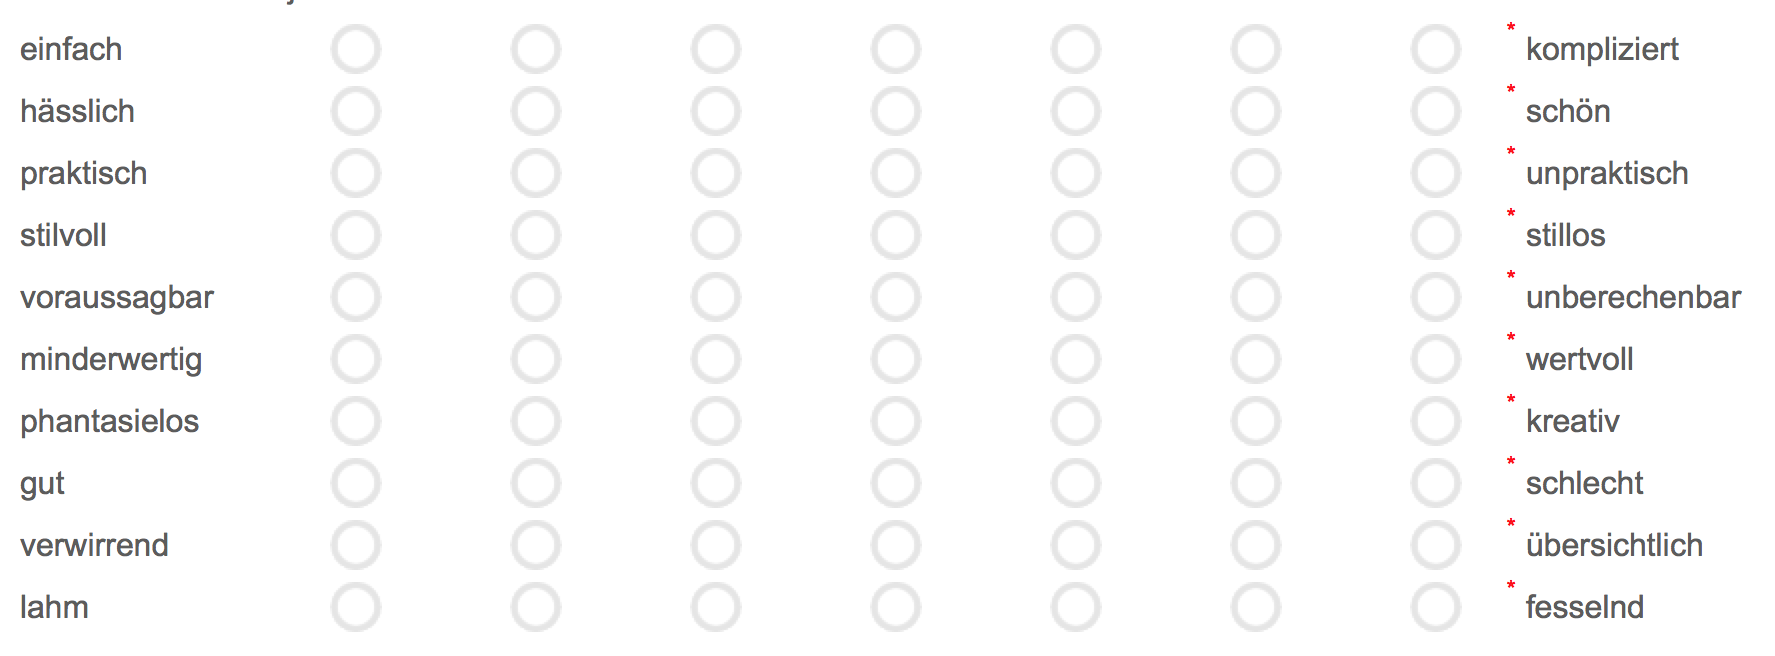
\includegraphics[width=1\textwidth]{grafiken/attrak_diff_short.png}
 \caption{AttrakDiff-Fragebogen}
 \label{fig:attrakDiffFragebogen}
\end{figure}
\section{Ergebnisse}
\subsection{Expertentest} \label{sec:resultExpert}
Es werden hier nur die Prinzipien der Heuristiken von Nielsen und Molich aufgeführt und begründet, die während der Auswertung nicht vollständig erfüllt wurden.\par
\heading{Aufgabe 1: Welche Länder werden als Höhenland eingestuft?}
% Wie Daten darstellen?
\textit{Schritt 1:} Auswählen des Anwendungsfalles \enquote{Land}\par
\textit{Schritt 2:} Auswählen des Attributes \enquote{Höhenland} für die Filterung\par
\begin{itemize}
 \item \textit{Ist die Lösung konsistent und hält Standards ein?} Standards werden eingehalten. Im Gegensatz zu der Navigationsleiste sind hier keine Tooltips für die Piktogramme vorhanden.
 \item \textit{Wird Erkennen Erinnern vorgezogen?} Die auswählbaren Kategorien sind mit sprechenden Piktogrammen versehen. Dennoch wären Tooltips von Vorteil für die korrekte Identifikation dieser.
\end{itemize}
\textit{Schritt 3:} Öffnen der Ergebnisansicht\par
\heading{Aufgabe 2a: Zeige die Datenübersicht von Deutschland an}\par
\textit{Schritt 1:} Auswählen des Anwendungsfalles \enquote{Land}\par
\textit{Schritt 2:} Auswählen des Attributes \enquote{Länderbenennung: Deutschland} für die Filterung\par
\textit{Schritt 3:} Öffnen der alternativen Ergebnisansicht (Galerie)\par
\heading{Aufgabe 2b: Exportiere diese als PDF}\par
\textit{Schritt 3:} Auswählen des Eintrages aus dem Navigation-Zusatzmenü (\ding{58}-Icon)\par
\begin{itemize}
 \item \textit{Wird Erkennen Erinnern vorgezogen?} Das \ding{58}-Icon taucht nach Wechsel in die Ergebnisansicht unter dem entsprechenden Element auf. Diese Änderung an einem normalerweise statischen Element wird u.U. durch den Benutzer nicht wahrgenommen.\par
\end{itemize}
\heading{Aufgabe 3: Welche Motoren werden in der Fahrzeugreihe \enquote{R8} der Marke \enquote{Audi} verbaut?}\par
\textit{Schritt 1:} Auswählen des Anwendungsfalles \enquote{Fahrzeug}\par
\textit{Schritt 2:} Filtern der Multi-Level-Liste nach der Bezeichnung \enquote{R8}\par
\textit{Schritt 3:} Alle Einträge auswählen\par
\begin{itemize}
 \item \textit{Wird versucht Fehler zu vermeiden?} Der Eintrag \textit{[alle Werte]} ist sichtbar, selbst wenn die Liste kein weiteres Element enthält. Dies kann den Nutzer schnell verwirren.\par
 \item \textit{Gibt es Unterstützung bei Fehlern?} Wenn es für den gewählten Schnellfiltertext keine Ergebnisse gibt, wird nur der Eintrag \textit{[Alle Werte angezeigt]}. Eine Hilfestellung zur Anzeige, dass keine Ergebnisse für den Schnellfiltertext gefunden wurden, wäre hilfreich.\par
\end{itemize}
\textit{Schritt 4:} Öffnen der Ergebnisansicht\par
\heading{Aufgabe 4: Welche Motoren werden in der Fahrzeugreihe \enquote{R8} der Marke \enquote{Audi} verbaut?}\par
\textit{Schritt 1:} Auswählen des Anwendungsfalles \enquote{Fahrzeug}\par
\textit{Schritt 2:} Auswählen der Marke Audi\par
\textit{Schritt 3:} Filtern der Multi-Level-Liste nach dem Motor \enquote{4,0L V8}\par
\textit{Schritt 4:} Auswählen aller gefundenen Einträge\par
\textit{Schritt 5:} Öffnen der Ergebnisansicht\par
\textit{Schritt 6:} Daten über \ding{58}-Menü der Navigationsleiste exportieren\par
\heading{Aufgabe 5a: Für welche Modelle des Fahrzeuges \enquote{Touran} der Marke \enquote{Volkswagen} existieren Freigaben sowohl in Deutschland, als auch in Österreich?}\par
\textit{Schritt 1:} Auswählen des Anwendungsfalles \enquote{LTÜ}\par
\textit{Schritt 2:} Auswählen des Fahrzeuges \enquote{Touran}\par
\textit{Schritt 3:} Wechsel zum Länder-Filter\par
\textit{Schritt 4:} Auswählen der Länder Deutschland und Österreich\par
\textit{Schritt 5:} Öffnen der alternativen Ergebnisansicht (Ergebnistabelle)\par
\heading{Aufgabe 5b: Welche Abgaskonzepte liegen den Modellen zugrunde?}\par
\textit{Schritt 1:} Abgaskonzept über Seitenleiste einblenden\par
\heading{Aufgabe 5c: Zeige nur die Abgaskonzepte an (Blende alle anderen Informationen aus).}\par
\textit{Schritt 1:} Abwählen aller Kategorien außer Abgaskonzept über Seitenleiste\par
\heading{Aufgabe 5d: Setze die Ansicht auf den Ursprungszustand zurück.}\par
\textit{Schritt 1:} Navigationsleiste auf Einstellungsmenü umschalten\par
\begin{itemize}
 \item \textit{Hat der Nutzer genügend Kontrolle und Freiheit?} Die Hauptnavigation ist vollständig ausgeblendet, damit die Einstellungsoptionen angezeigt werden können\par
 \item \textit{Sind Hilfe und Dokumentation vorhanden?} Es ist keine Hilfe für diese sekundären Funktionen verfügbar\par
\end{itemize}
\textit{Schritt 2:} Betätigen der \enquote{Ergebniskonfiguration zurücksetzen}- Schaltfläche\par
\heading{Aufgabe 6a: In welchen Ländern existiert eine Freigabe für das Modell mit der Fahrzeugbezeichnung \enquote{VW216/0EU\_{}K T-Cross} und der Abgas-Prüfnummer (Abgas PrNr) \enquote{7GM}}\par
\textit{Schritt 1:} Auswählen des Anwendungsfalles \enquote{LTÜ}\par
\textit{Schritt 2:} Auswählen des Fahrzeuges mit der Bezeichnung \enquote{VW216/0EU\_{}K T-Cross} für die Filterung\par
\textit{Schritt 3:} Öffnen der Ergebnisansicht (Listenansicht)\par
\begin{itemize}
 \item \textit{Gibt es Unterstützung bei Fehlern?} Wenn kein Fahrzeug selektiert ist oder keine Freigabe für das ausgewählte Fahrzeug existiert, wird die rechte Tabelle leer angezeigt. Hinweise wären hier für den Benutzer hilfreich.\par
 \item \textit{Sind Hilfe und Dokumentation vorhanden?} Der Hilfetext ist allgemeingültig gehalten und unterstützt nicht bei der Verwendung dieser speziellen Ergebnisansicht\par
\end{itemize}
\textit{Schritt 4:} Einblenden der Kategorie \enquote{Abgas} über die Seitenleiste\par
\textit{Schritt 5:} Filter in Kopfzeile der Spalte Abgas-Prüfnummer öffnen, alles deselektieren außer Wert \enquote{7GM}\par
\begin{itemize}
 \item \textit{Gibt es Unterstützung bei Fehlern?} Werden alle Einträge im Filter deselektiert, wird eine leere Tabelle angezeigt. Ein Hinweis für den Benutzer wäre hier hilfreich.\par
 \item \textit{Sind Hilfe und Dokumentation vorhanden?} Der Hilfetext gibt keinen Aufschluss über die Funktion des Filters in den Spaltenköpfen.\par
\end{itemize}
\textit{Schritt 6:} Verbleibendes Fahrzeugmodell selektieren \par
\heading{Aufgabe 6b: Betrachte die Details einer Freigabe des Modells.}\par
\textit{Schritt 1:} Doppelklick auf eine der angezeigten Länderfreigaben\par
\heading{Aufgabe 7: Welche Modelle des Fahrzeuges \enquote{S1} der Marke \enquote{Audi} haben eine Motorfreigabe für Deutschland.}\par
\textit{Schritt 1:} Auswählen des Anwendungsfalles \enquote{LTÜ}\par
\textit{Schritt 2:} Auswählen der Marke \enquote{Audi}\par
\textit{Schritt 3:} Filterung der Fahrzeuge nach der Bezeichnung \enquote{S1}\par
\textit{Schritt 4:} Auswählen aller Werte\par
\textit{Schritt 5:} Wechsel zu Länder-Filter\par
\textit{Schritt 6:} Auswählen der Länderbezeichnung Deutschland\par
\textit{Schritt 7:} Öffnen der alternativen Ergebnisansicht (Ergebnistabelle)\par
\subsection{Nutzertests} \label{sec:resultUser}
Es werden nur die gefundenen Probleme aufgeführt, die Nutzer bei der Bedienung hatten.
\heading{Aufgabe 1: Welche Länder werden als Höhenland eingestuft?}
\begin{itemize}
 \item Versucht, genau das \textbf{-} -Symbol beim Deselektieren von Filterkriterien zu treffen
 \item Gewählte Filterkriterien in Seitenleiste nicht als klickbar erkannt (zwecks Deselektierung)
 \item Versucht, über Texteingabe im Kopfzeilenfilter der Ergebnisansicht zu scrollen
\end{itemize}
\heading{Aufgabe 2: Zeige die Datenübersicht von Deutschland an.}
\begin{itemize}
 \item Versucht, die Galerie im Hintergrund zu bedienen, nachdem der Lesemodus versehentlich geöffnet wurde
 \item Das \ding{58}-Icon in der Navigationsleiste ist schwierig zu treffen, oft das Menüitem selbst angeklickt
 \item \ding{58}-Icon oft nicht wahrgenommen
 \item Scrollen in Tabelle über Tippen des Namens versucht (wie bereits in Galerie implementiert)
\end{itemize}
\heading{Aufgabe 3: Welche Motoren werden in der Fahrzeugreihe \enquote{R8} der Marke \enquote{Audi} verbaut?}
\begin{itemize}
 \item Eintrag \textit{[Alle Werte]} nicht wahrgenommen
 \item Versucht, in der Multi-Level-Liste mehrere Einträge per Shift zu selektieren
\end{itemize}
\heading{Aufgabe 4: Exportiere eine Excel-Übersicht über alle Fahrzeugmodelle der Marke \enquote{Porsche}, die einen \enquote{4.0L V8} Motor verbaut haben.}
\begin{itemize}
 \item Länderfilter nicht auf Anhieb gefunden
 \item Versucht, \textit{F11} als Schnelltaste für Vollbildmodus zu benutzen
 \item Sortierung der Ländernamen in Multi-Level-Liste verwirrend (nach interner Schlüsselnummer)
 \item Verwirrung durch fehlenden Text in der Listenansicht des LTÜ-Anwendungsfalles, wenn es für das selektierte Fahrzeug keine Länderfreigaben gibt
 \item Unterkategorien bei Subnavigation in LTÜ-Detailansicht nicht offensichtlich (LTÜ und Motorfreigabe)
 \item Meist Benutzung der Navigationselemente zum Verlassen der Detailansicht
\end{itemize}
\heading{Aufgabe 5: Zeige alle Motorfreigaben der Fahrzeugreihe \enquote{S1} in Deutschland an.}
\begin{itemize}
 \item Das Motorfreigabe-Icon wurde nicht auf Anhieb erkannt
 \item Verwirrung beim Entfernen von Kategorien aus der Filterselektion (Eimer-Icon benötigt zwei Klicks zum Ausführen der Aktion)
\end{itemize}
\heading{Aufgabe 6: Setze alle Einstellungen und geladenen Daten zurück.}
\begin{itemize}
 \item Button zum Zurücksetzen der Daten als \enquote{Aktualisieren} erkannt (aufgrund von Icon und irreführendem Tooltip)
\end{itemize}
\heading{Generelle Erkenntnisse}
\begin{itemize}
 \item Hilfetexte wurden nicht betrachtet
 \item Schnellfilter in Multi-Level-Liste erst spät wahrgenommen
 \item Wenige Erstnutzer machten Gebrauch von Mnemonics, Gesten- oder Tastursteuerung
\end{itemize}